% fancytikzposter.tex, version 2.1
% Original template created by Elena Botoeva [botoeva@inf.unibz.it], June 2012
% 
% This file is distributed under the Creative Commons Attribution-NonCommercial 2.0
% Generic (CC BY-NC 2.0) license
% http://creativecommons.org/licenses/by-nc/2.0/ 


\documentclass{a0poster}

\usepackage{fancytikzposter} 


%%%%% --------- Change here if you want ---------- %%%%%
%% margin for the geometry package, must be changed before using the geometry package
%% default value is 4cm
 \setmargin{1}

%% the space between the blocks
%% default value is 2cm
 \setblockspacing{1.15}

%% the height of the title stripe in block nodes, decrease it to save space
%% default value is 3cm
 \setblocktitleheight{2}

%% the number of columns in the poster, possible values 2,3
%% default value is 2
% \setcolumnnumber{2}

%% the space between two or more groups of authors from different institutions
%% used in \maketitle
% \setinstituteshift{10}

%% which template to use
%% N1 simple, standard look, with a colored background and gray boxes
%% N2 board with nodes
%% N3 another standard look
%% N4 envelope-like look
%% N5 with a wave-like head, original idea taken from
%%%% http://fc09.deviantart.net/fs71/f/2010/322/1/1/scientific_poster_by_nabuy-d333ria.jpg
%\usetemplate{6}

%% components of the templates
%% (the maximal possible numbers are mentioned as the parameters)
% \usecolortemplate{4}
% \usebackgroundtemplate{5}
% \usetitletemplate{2}
% \useblocknodetemplate{5}
% \useplainblocktemplate{4}
% \useinnerblocktemplate{2}


%% the height of the head drawing on top 
%% applicable to templates N3, 4 and 5
% \setheaddrawingheight{14}


%% change the basic colors
%\definecolor{myblue}{HTML}{008888} 
%\setfirstcolor{myblue}% default 116699
%\setsecondcolor{gray!80!}% default CCCCCC
%\setthirdcolor{red!80!black}% default 991111

%% change the more specific colors
% \setbackgrounddarkcolor{colorone!70!black}
% \setbackgroundlightcolor{colorone!70!}
% \settitletextcolor{textcolor}
% \settitlefillcolor{white}
% \settitledrawcolor{colortwo}
% \setblocktextcolor{textcolor}
% \setblockfillcolor{white}
% \setblocktitletextcolor{colorone}
% \setblocktitlefillcolor{colortwo} %the color of the border
% \setplainblocktextcolor{textcolor}
% \setplainblockfillcolor{colorthree!40!}
% \setplainblocktitletextcolor{textcolor}
% \setplainblocktitlefillcolor{colorthree!60!}
% \setinnerblocktextcolor{textcolor}
% \setinnerblockfillcolor{white}
% \setinnerblocktitletextcolor{white}
% \setinnerblocktitlefillcolor{colorthree}




%%% size of the document and the margins
%% A0
% \usepackage[margin=\margin cm, paperwidth=118.9cm, paperheight=84.1cm]{geometry} 
%\usepackage[margin=\margin cm, paperwidth=84.1cm, paperheight=118.9cm]{geometry}

%% A1 portrait
\usepackage[margin=\margin cm, paperwidth=59.4cm, paperheight=84.1cm]{geometry}


%% B1
% \usepackage[margin=\margin cm, paperwidth=70cm, paperheight=100cm]{geometry}



%% changing the fonts
\usepackage{cmbright}
%\usepackage[default]{cantarell}
%\usepackage{avant}
%\usepackage[math]{iwona}
\usepackage[math]{kurier}
\usepackage[T1]{fontenc}


%% add your packages here
\usepackage{hyperref}





\title{COMBINE (ISCB RSG Australia)\\combine.org.au}
\author{Committee: Benjamin Goudey (\emph{President}),
        Karin Klotzbuecher (\emph{Secretary}),\\
        {\bf Sabrina Rodrigues,
        Andrew Lonsdale,
        Thomas Coudrat, Scott Ritchie, Marek Cmero,
        Kian Ho}}
       



\begin{document}
 %% a plain block
  %% #1 - rotate angle (optional), #2 - where, #3 - width, #4 - title, #5 - text
  %%%%%%%%%% ------------------------------------------ %%%%%%%%%%
  
%%%%% ---------- the background picture ---------- %%%%%
%% to change it modify the macro \BackgroundPicture
\ClearShipoutPicture
\AddToShipoutPicture{\BackgroundPicture}

\noindent % to have the picture right in the center
\begin{tikzpicture}
  \initializesizeandshifts
  % \setxshift{15}
  % \setyshift{2}


  %% the title block, #1 - shift, the default value is (0,0), #2 - width, #3 - scale
  %% the alias of the title block is `title', so we can refer to its boundaries later
  \ifthenelse{\equal{\template}{1}}{ 
    \titleblock{47}{1}
  }{
    \titleblock{47}{1.5}
  }

  %% a logo can be added to the title block
  %% #1 - anchor relative to the title block, #2 - shift, #3 - width, #3 - file name
  % \ifthenelse{\equal{\template}{2}}{ 
  %   \addlogo[south west]{(2,0)}{6cm}{unibz_b.png}
  % }{
  %   \addlogo[south west]{(2,0)}{6cm}{unibz_w.png}
  % }


  %% a block node, with the specified position (optional), title and the content
  %% #1 - where (optional), #2 - title, #3 - text
  %%%%%%%%%% ------------------------------------------ %%%%%%%%%%
  \blocknode{About Us}%
  {
        \begin{center}
        
        
\includegraphics[width=0.5\linewidth]{./images/COMBINE-logo.png}
   
        \end{center}
    \textbf{COMBINE} is a student-run Australian organisation for researchers in
    \textbf{computational biology}, \textbf{bioinformatics}, and related
    fields.\\[2ex]
    We aim to bring together students and early-career
    researchers from the computational and life sciences for networking,
    collaboration, and professional development.\\
    }

  \blocknode{ISCB Affiliation}%
  {
  \begin{minipage}[c]{\linewidth}
  

    \textbf{COMBINE} is the official
    International Society for\\ Computational Biology (ISCB) Regional Student Group for
    Australia.

    \vspace{3ex}

    \begin{minipage}[c]{\linewidth}
        \centering
    \begin{minipage}[c]{0.47\linewidth}
        \centering
        
\includegraphics[width=0.85\linewidth,valign=M]{./images/iscb_logo.png}\\[1ex]
        
\includegraphics[width=0.85\linewidth,valign=M]{./images/ISCBSC-logo.png}
    \end{minipage}
    ~
    \begin{minipage}[c]{0.33\linewidth}
        \centering
        
\includegraphics[scale=0.25]{./images/RSGAU-logo.png}
    \end{minipage}
    \end{minipage}

    \vspace{3ex}

    \begin{itemize}
        \item 25 ISCB Regional Student Groups (RSGs) around the world.
        \item Student council symposiums at ISCB conferences:
        \begin{itemize}
        
        \item ISMB2014 - July 11--15, 2014 in Boston, USA.
        \item ECCB2014 - September 7--10, 2014 in Strasbourg, France.
    \end{itemize}
    \end{itemize}

\end{minipage}
  }

  %%%%%%%%%% ------------------------------------------ %%%%%%%%%%
  \blocknode{Previous COMBINE Events}%
  {  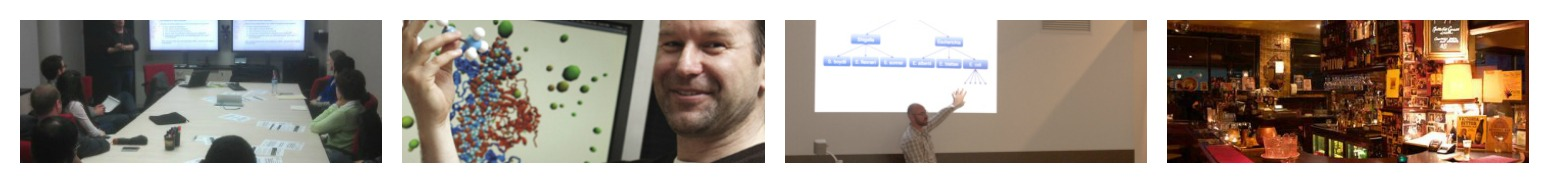
\includegraphics[width=1\linewidth]{./images/COMBINE-collage.jpg}
    \bp{\bfseries Alignment free methods for sequence comparison}\\ (seminar)\\
    Dr.~Tom Conway, NICTA\\[1ex]
    \bp{\bfseries How to get your computer to freeze} (seminar)\\
    Dr.~Mike Kuiper, VLSCI\\[1ex]
    \bp{\bfseries How to give a better research presentation} (workshop)\\
    Prof. Justin Zobel, Uni.~Melb.\\[1ex]
    \bp{\bfseries Python for the Life Sciences} (workshop)\\
    Dr.~Bernie Pope, VLSCI\\[1ex]
   \bp{\bfseries Wikipedia edit-a-thon \& Pizza Lunch} (workshop/social)\\
	Drs. Gayle Philip, Bernie Pope, and Geoff Macintyre.\\
	\begin{center}
	
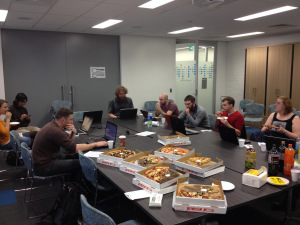
\includegraphics[height=45mm]{./images/wiki1.jpg}  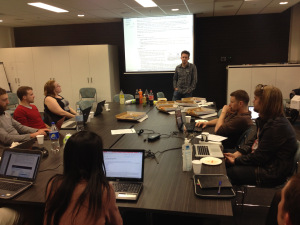
\includegraphics[height=45mm]{./images/wiki2.jpg}  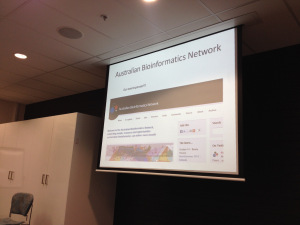
\includegraphics[height=45mm]{./images/abn.jpg}
    
	\end{center}
	%
  }


  %%%%%%%%%%%%% NEW COLUMN %%%%%%%%%%%%%%% 
  \startsecondcolumn 




  %% by default, the position of the new block node is right below the previous
  %% block node, stored in (currenty)
  %% box is the alias of the previous block, so we can refer to its boundaries

  %%%%%%%%%% ------------------------------------------ %%%%%%%%%%
  \blocknode{Annual Symposium}%
  {
The COMBINE Student Symposium  is an opportunity for students and early-career researchers in computational biology, bioinformatics, and the life sciences to share their research with others in these fields.\\

\begin{center}
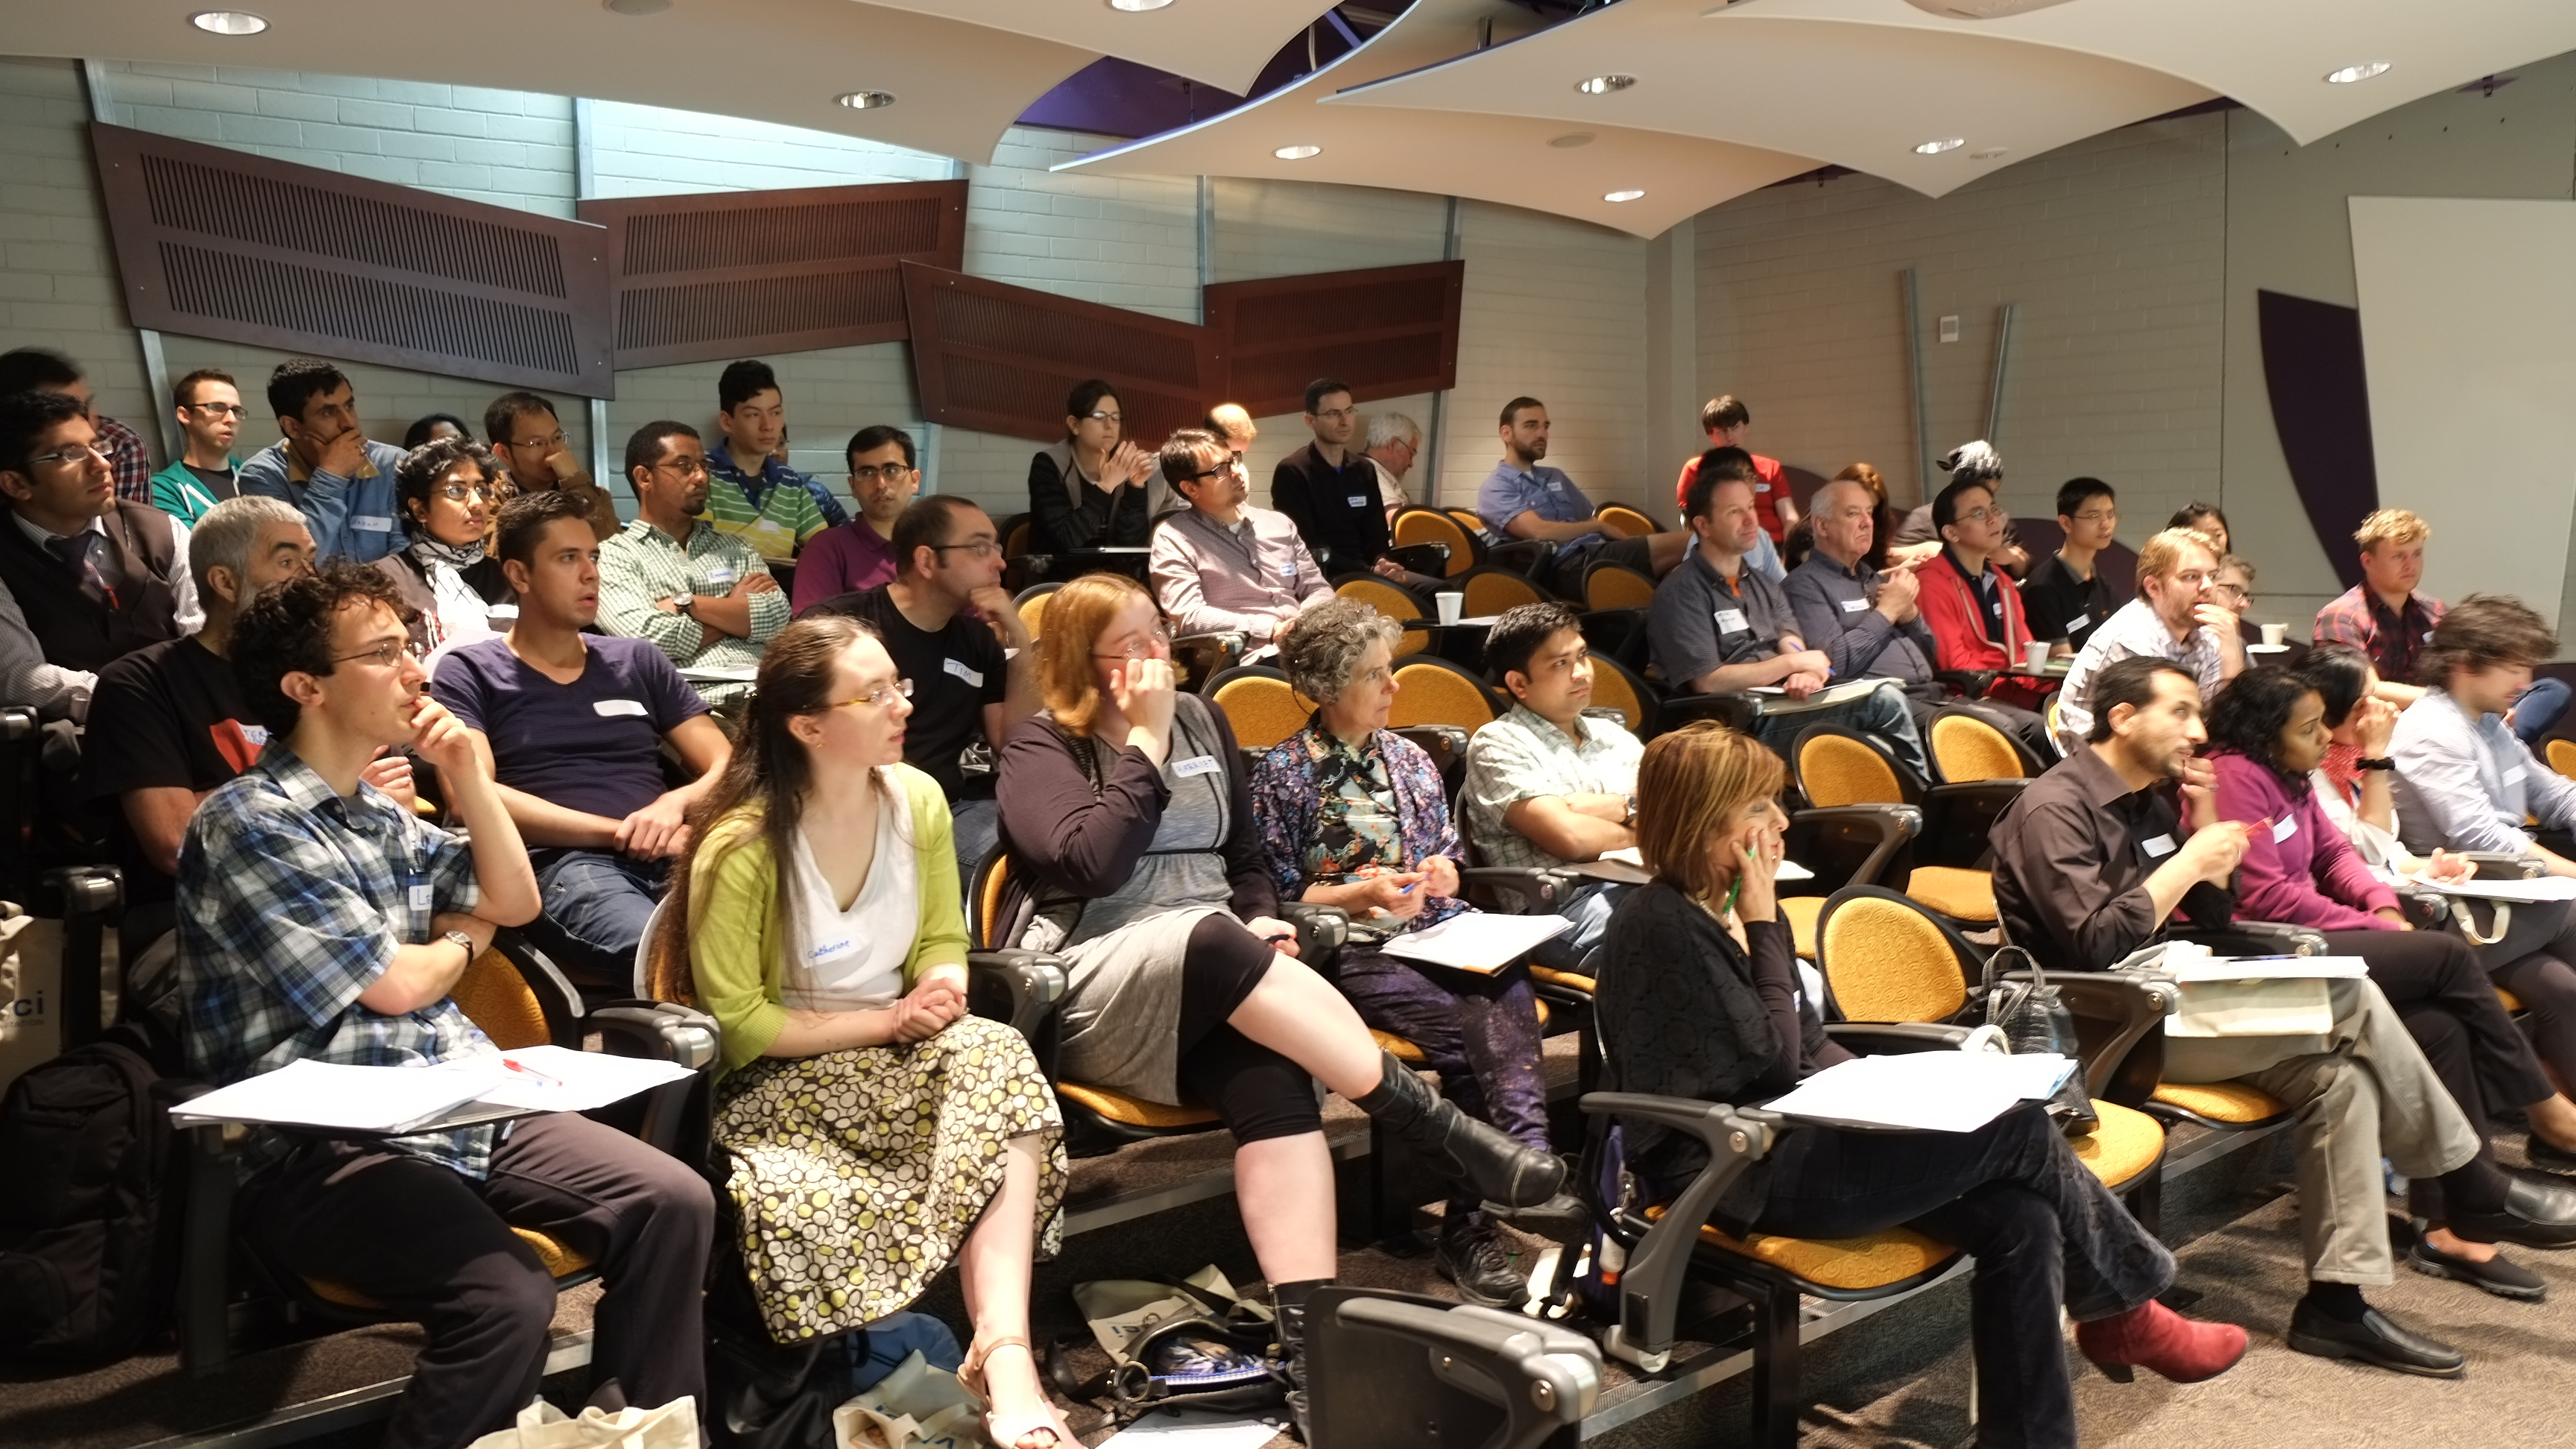
\includegraphics[height=40mm]{./images/aud.JPG}
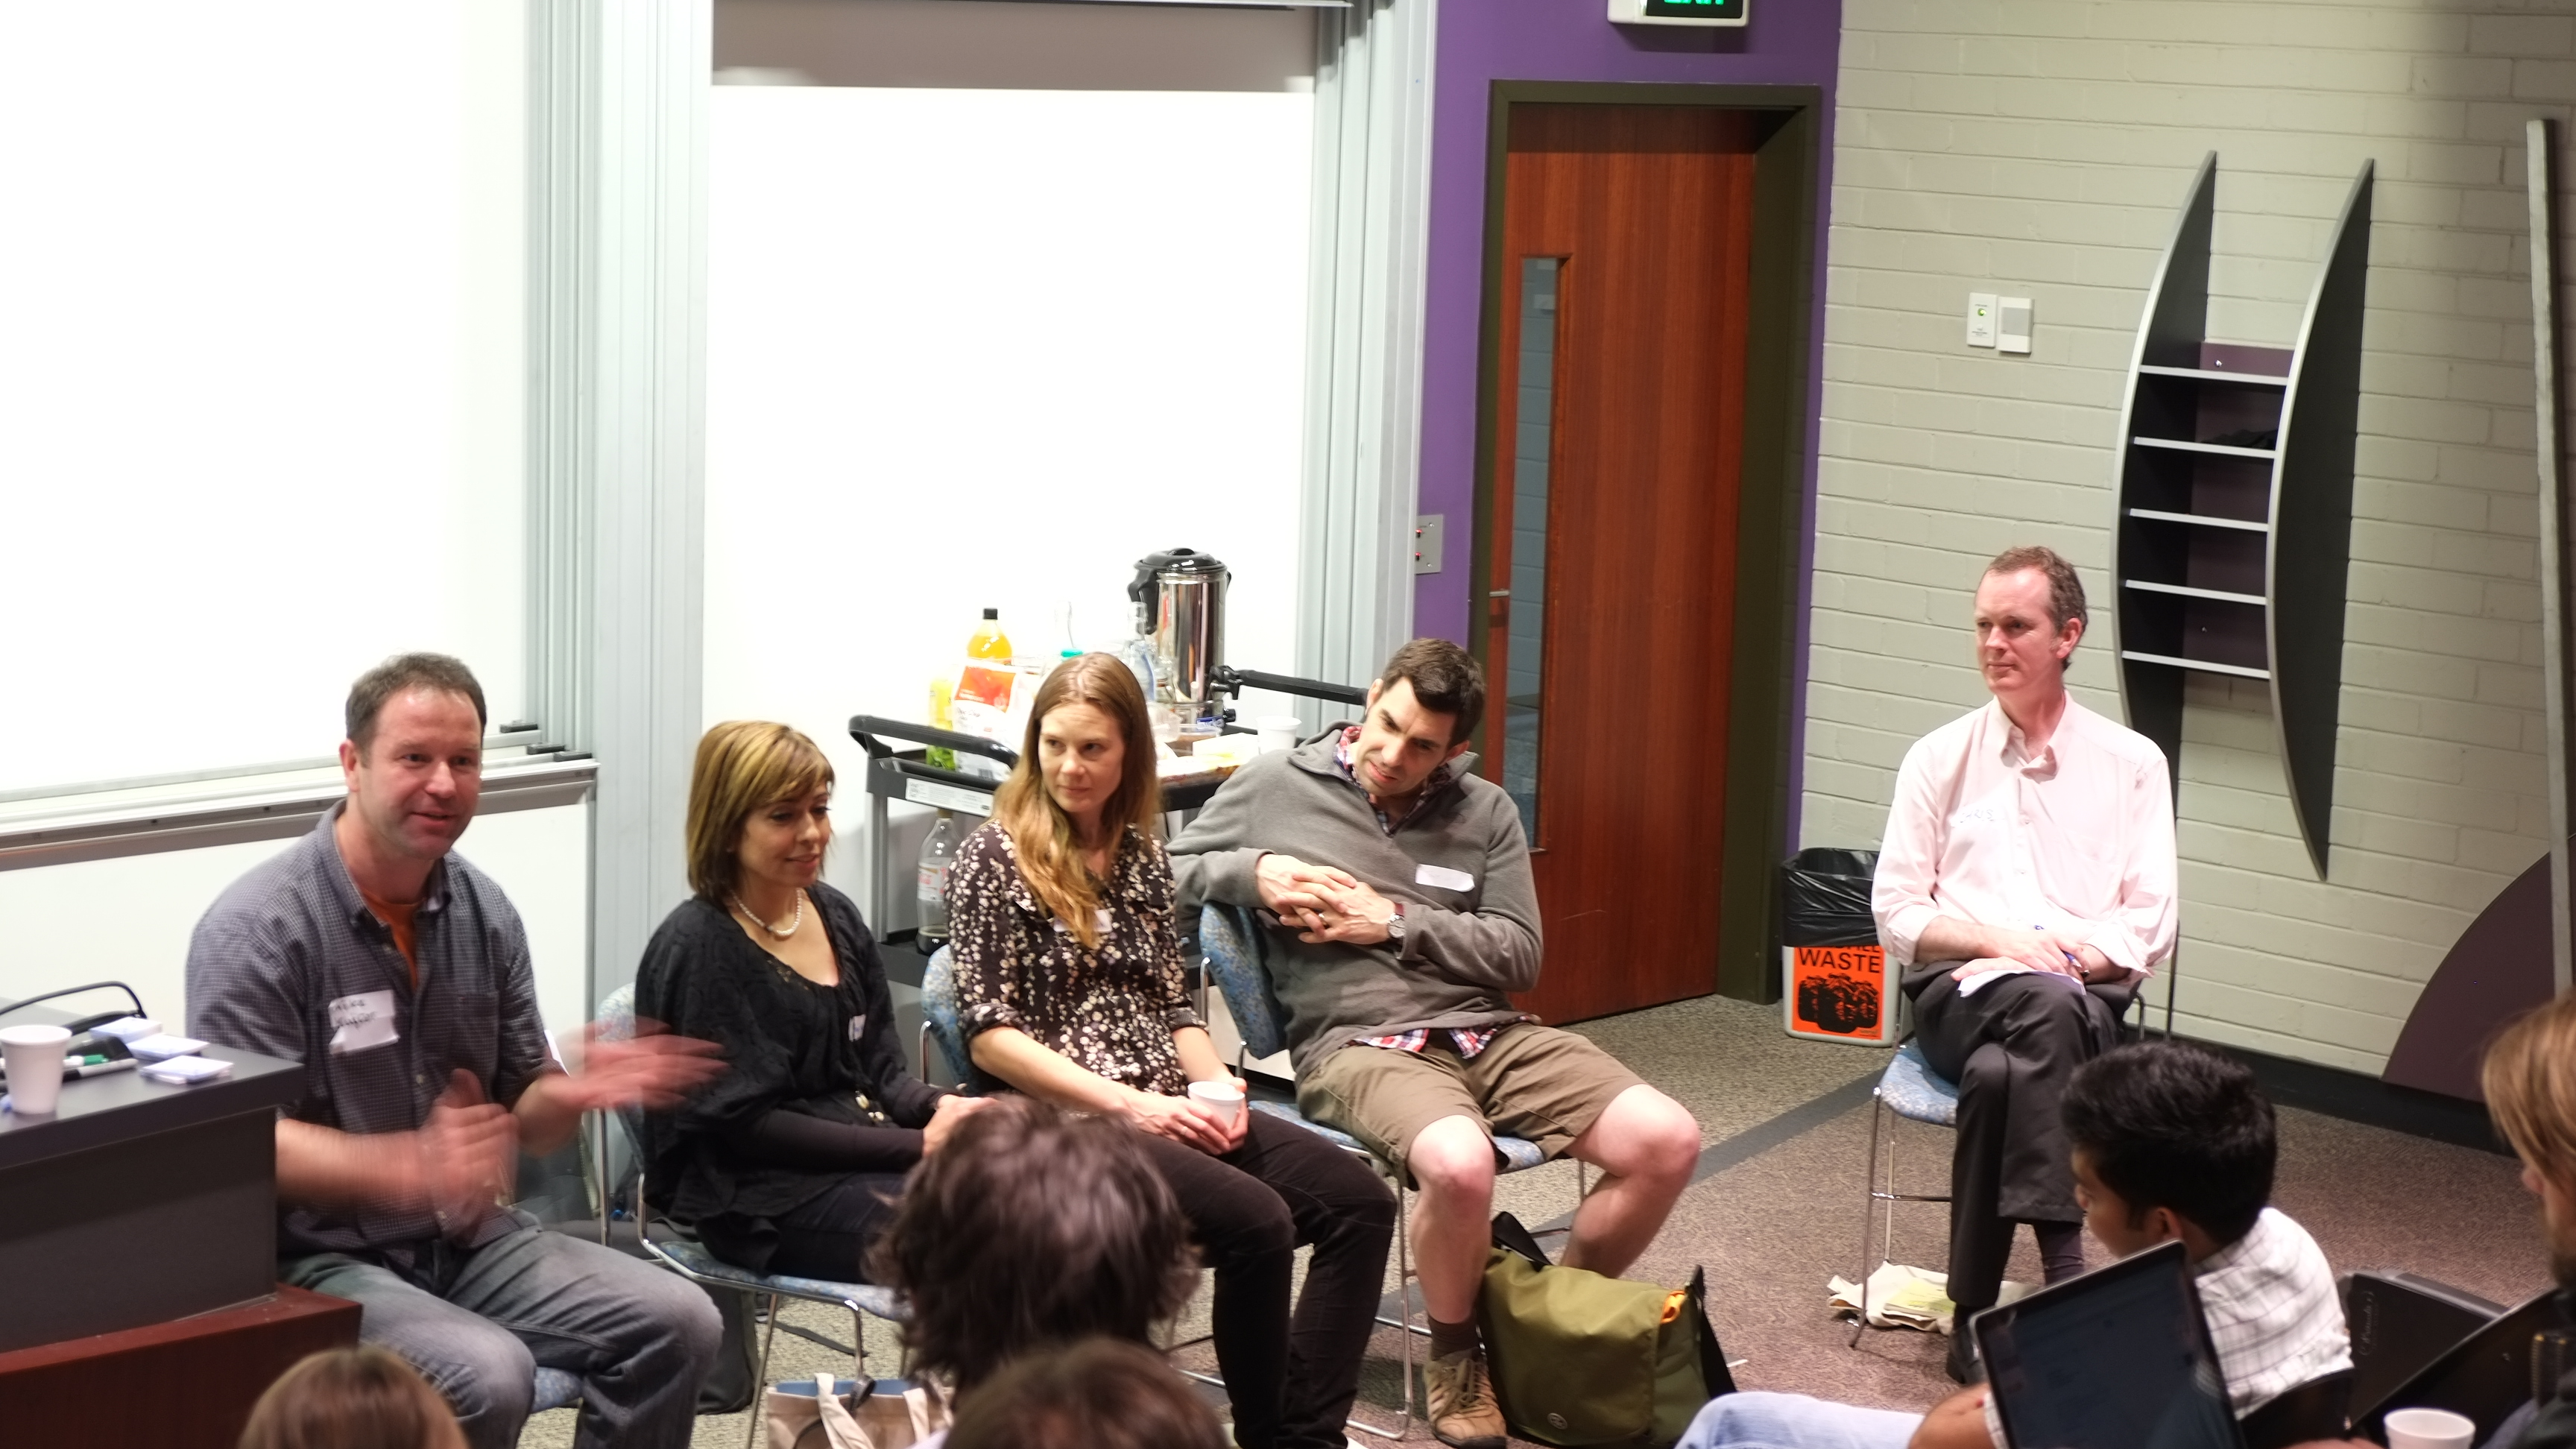
\includegraphics[height=40mm]{./images/qa.JPG}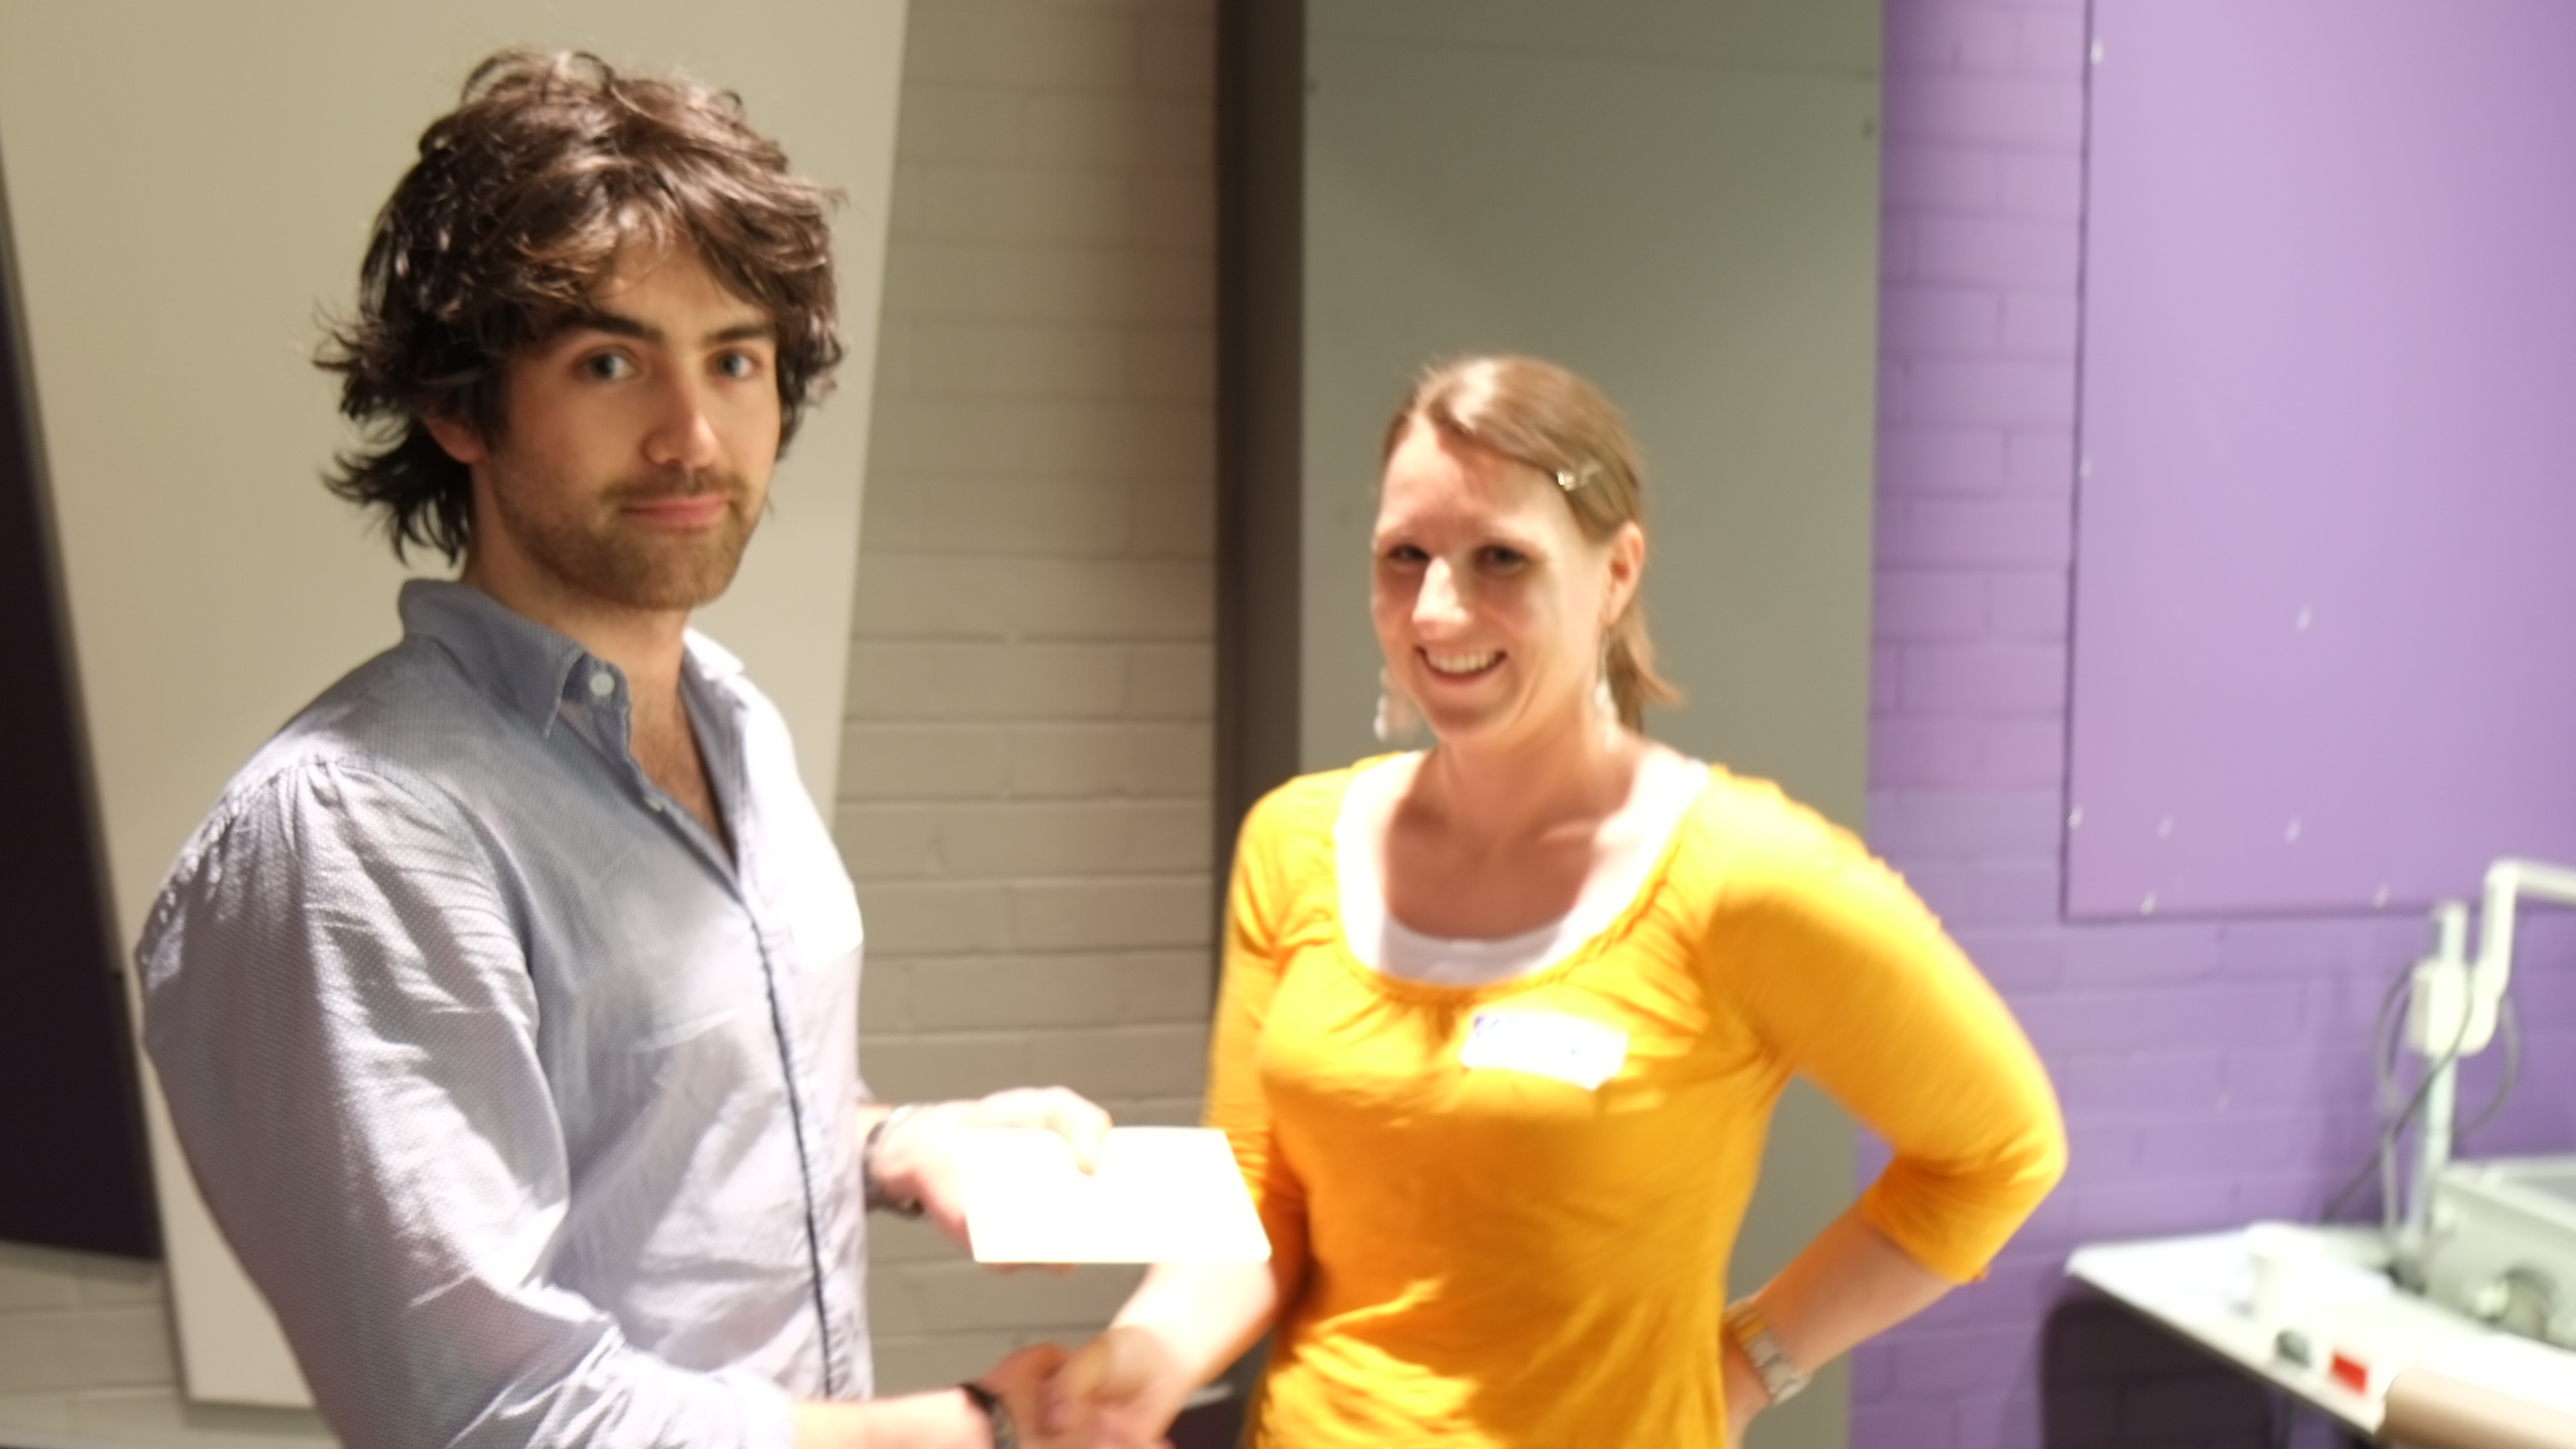
\includegraphics[height=40mm]{./images/win.JPG}
\end{center}

Symposium 2013 included over 50 attendees, a careers panel and prizes for the winning presentations.
  }
  
   
  \blocknode{Join Us!}%
  {
   \begin{itemize}
    	\item Contact us for assistance in organsing workshops,\\ seminars and social events in your area.
        \item We are currently looking for volunteers to join our\\ committee.
        \item Present your work at a COMBINE event before\\ attending conferences!
        \item Are you an expert on $x$? Give a workshop on $x$!
    \end{itemize}
    \vspace{1ex}

  \raisebox{-.25\height}{
\includegraphics[height=15mm]{./images/facebooklogo.png}} \bp{facebook.com/combine.australia}\\[2ex]
 \raisebox{-.25\height}{
\includegraphics[height=15mm]{./images/twitter-logo.png}} \bp{twitter.com/combine\_au}\\[2ex]
    For more information, email \textit{combine@combine.org.au} or 
visit\\ \textbf{combine.org.au}
  }
  
    \blocknode{Sponsors}%
  {

  We are proudly sponsored by:\\[1ex]
\begin{center}

    \centering
    
\includegraphics[height=30mm]{./images/ICT-for-Life-Sciences-Forum-logo.png}\quad
    
\includegraphics[height=30mm]{./images/ISCBSC-logo.png}
    \end{center}
    \vspace{2ex}
    
  
  }


 \blocknode{Poster}%
  {  
  Poster based on template by Elena Botoeva\\ \textit{http://www.inf.unibz.it/{\textasciitilde}ebotoeva/fancytikzposter.html}
}
  
  

  %% to place the next node centered vertically in the second column, we can
  %% obtain the y-coordinate of the previous node using macro
  %% \getcurrentrow{note}, where note is the alias of the callout node, and
  %% then specify the coordinate of the next node using coordinate (currentrow)
  \getcurrentrow{note}



 
  %% the coordinate (currenty) is used in the default placing of the next blocknode
 \getcurrentrow{note}
 \coordinate (currenty) at ($(currentrow)+(xshift)-(yshift)$);



   %%%%%%%%%%%%% NEW COLUMN %%%%%%%%%%%%%%% 
  %% (if column number is 3)
  \startthirdcolumn

 \end{tikzpicture}





\end{document}




